\documentclass[11pt]{article}
\usepackage[T1]{fontenc}
\usepackage[french]{babel}
\usepackage{csquotes}
\usepackage[margin=2.5cm]{geometry}
\usepackage{amsmath, amssymb, amsthm}
\usepackage{graphicx}
\usepackage{booktabs}
\usepackage[style=numeric, sorting=none]{biblatex}
\addbibresource{references.bib}
\usepackage[colorlinks=true, allcolors=blue]{hyperref}

\newtheorem{theoreme}{Théorème}
\newtheorem{lemme}[theoreme]{Lemme}
\theoremstyle{definition}
\newtheorem{definition}[theoreme]{Définition}

\title{{{TITLE}}}
\author{%
  {{AUTHOR}}\thanks{Département, Établissement, Ville, Pays.
    Courriel~: \href{mailto:prenom.nom@exemple.org}{prenom.nom@exemple.org}.}%
}
\date{\today}

\begin{document}

\maketitle

\begin{abstract}
Le résumé présente en un paragraphe la question étudiée, la méthode, les
principaux résultats et leur portée. La plupart des revues en limitent la
longueur à 150 ou 250 mots.

\medskip
\noindent\textbf{Mots-clés:} premier mot-clé, deuxième mot-clé, troisième
mot-clé.
\end{abstract}

\section{Introduction}
\label{sec:introduction}

L'introduction situe le problème, résume les travaux antérieurs
\parencite{knuth1981, lamport1994} et annonce la contribution de l'article. La
section~\ref{sec:methode} décrit la méthode, la section~\ref{sec:resultats}
présente les résultats et la section~\ref{sec:conclusion} conclut.

\section{Méthode}
\label{sec:methode}

\begin{definition}
Une suite $(u_n)$ de nombres réels est \emph{bornée} s'il existe un réel $M$
tel que $\lvert u_n \rvert \le M$ pour tout entier $n$.
\end{definition}

\begin{theoreme}[Bolzano-Weierstrass]
\label{thm:bw}
Toute suite réelle bornée admet une sous-suite convergente.
\end{theoreme}

\begin{proof}
On découpe l'intervalle $[-M, M]$ en deux moitiés, dont l'une contient une
infinité de termes de la suite, puis on recommence dans cette moitié. Les
intervalles emboîtés ainsi obtenus définissent la limite d'une sous-suite.
\end{proof}

Le modèle étudié s'écrit
\begin{equation}
  \label{eq:modele}
  y_i = \beta_0 + \beta_1 x_i + \varepsilon_i, \qquad i = 1, \dots, n,
\end{equation}
où les erreurs $\varepsilon_i$ sont indépendantes et de moyenne nulle.

\section{Résultats}
\label{sec:resultats}

Le tableau~\ref{tab:resultats} donne les coefficients estimés du
modèle~\eqref{eq:modele} et la figure~\ref{fig:donnees} en illustre
l'ajustement.

\begin{table}[htbp]
  \centering
  \caption{Coefficients estimés.}
  \label{tab:resultats}
  \begin{tabular}{lrrr}
    \toprule
    Coefficient & Estimation & Écart-type & Valeur $p$ \\
    \midrule
    $\beta_0$ & 1,24 & 0,31 & $< 0{,}001$ \\
    $\beta_1$ & 0,87 & 0,12 & $< 0{,}001$ \\
    \bottomrule
  \end{tabular}
\end{table}

\begin{figure}[htbp]
  \centering
  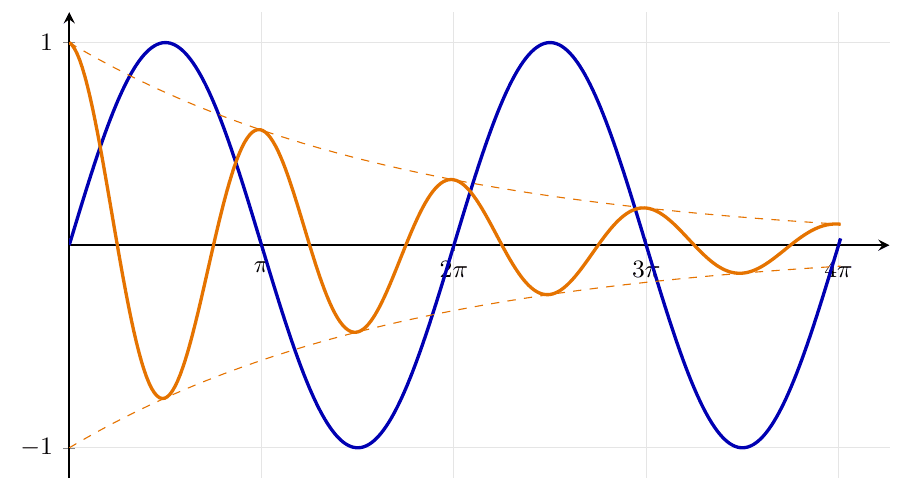
\includegraphics[width=0.7\linewidth]{images/courbes.png}
  \caption{Une image du projet: remplacez-la par la vôtre.}
  \label{fig:donnees}
\end{figure}

\section{Conclusion}
\label{sec:conclusion}

La conclusion rappelle les résultats et ouvre sur les travaux à venir
\parencite{mittelbach2023}.

\section*{Remerciements}

Les auteurs remercient les organismes qui ont financé ces travaux.

\printbibliography

\end{document}
